\documentclass{article} % defines the type of document
\usepackage{indentfirst} % this package causes the first paragraph of each section to be indented
\usepackage{graphicx} % Required for inserting images
\usepackage{csvsimple} % this package allows reading CSV
\usepackage{longtable} % this package allows tables to be too long for one page (taking up more than one)
\usepackage{amsmath} % For matrix notation etc
\usepackage{caption} % This package allows customization of captions in tables and figures
\captionsetup[table]{labelformat=empty} % remove automatic numbering of table captions
\captionsetup[table]{justification=centering} % center table captions
\usepackage{hyperref} %  Package for adding hyperlinks within the document
\usepackage{float} % To keep the image fixed and text after it (bypass latex optimization) [H]

\title{Econometrics - Revisiting and developing (in progress)} % Set the document title
\author{Thiago  Vinicius Gomiero} % Define the document author
\date{February 2024} % Defines the date that appears in the document

\begin{document} % This command indicates the beginning of the document content.


\maketitle % This command creates the previously defined document title, author and date

\section{Introduction} % This command creates a section with the title "Introduction"
% The following text is the content of the "Introduction" section.
The linear regression analysis is based on the book I used, \href{https://drive.google.com/file/d/1TIP3vEfFTzmsyAT_NdfeEucQ3Buzl79L/view?usp=sharing}{Econometric Methods by Jack Johnston}, and the class notes from \href{https://1drv.ms/o/s!AmlxSSt9Wu45_hK-coxj_ULKBVLC?e=dclINF}{Econometrics 1} (and possibly 2) that I took at FEA-USP.

Several excerpts have been rewritten/adapted based on the main book (and class notes) with the aim of developing my writing skills in R and LaTeX.

Most of the statistical calculations were carried out in Rstudio with the same objective. Excel was also used to clean the database and integrate with Rstudio.

I will try to use some techniques and concepts presented in Quantitative Economics with R; A Data Science Approach\href{https://link.springer.com/book/10.1007/978-981-15-2035-8}{link}. Its PDF can be easily found by searching online.

The main objective here will not be to present a formal approach to econometrics. Instead, I will aim to provide a concise overview of the theory necessary to understand the topic, and proceed with practical examples using R, Excel, and other tools.


\section{The base of Linear Rgression}
To understand Linear Regression, we need to grasp some statistical concepts.
Let's start with relationships between two variables.
\subsection{Bivariate Frequency Distribution}
% latex table generated in R 4.3.2 by xtable 1.8-4 package
% Fri Feb  2 17:17:34 2024
\begin{table}[H]
\centering
\textbf{Note:} The columns refer to chest circumference (inches), and the rows refer to height (inches)
\begin{tabular}{rrrrrrr}
  \hline
 & 33-35 & 36-38 & 39-41 & 42-44 & 45-over & Row totals \\ 
  \hline
64-65 & 39.00 & 331.00 & 326.00 & 26.00 & 0.00 & 722.00 \\ 
  66-67 & 40.00 & 591.00 & 1010.00 & 170.00 & 4.00 & 1815.00 \\ 
  68-69 & 19.00 & 312.00 & 1144.00 & 488.00 & 18.00 & 1981.00 \\ 
  70-71 & 5.00 & 100.00 & 479.00 & 290.00 & 23.00 & 897.00 \\ 
  72-73 & 0.00 & 17.00 & 120.00 & 153.00 & 27.00 & 317.00 \\ 
  Column totals & 103.00 & 1351.00 & 3079.00 & 1127.00 & 72.00 & 5732.00 \\ 
   \hline
\end{tabular}
\end{table}
% latex table generated in R 4.3.2 by xtable 1.8-4 package
% Fri Feb  2 17:48:42 2024
\begin{table}[H]
\centering
\textbf{Note:} The second table displays conditional means
\begin{tabular}{rrrrrr}
  \hline
 & 1 & 2 & 3 & 4 & 5 \\ 
  \hline
mean of height given chest-inches  & 66.31 & 66.84 & 67.89 & 69.16 & 70.53 \\ 
  mean of chest given height-inches & 38.41 & 39.19 & 40.26 & 40.76 & 41.80 \\ 
   \hline
\end{tabular}
\end{table}
The second table shows a lot of numbers. But how were they calculated?
Let's demonstrate that:
The number 66.84 in the first row, second column of the second table was derived by performing the following calculation:
\begin{math}(64.5\cdot331+66.5\cdot591+68.5\cdot312+70.5\cdot100+72.5\cdot17)/1351=66.84\end{math}.

In a similary way, the number 38.41 in the second row, first column of the second table:
\begin{math}(39\cdot34+331\cdot37+326\cdot40+26\cdot43)/722 = 38.41\end{math}

\subsection{The correlation coefficient}
 The correlation coefficient measures the direction and closeness of the linear association between two variables.
Let´s denote the observations by \begin{math}(X_i, Y_i)\end{math} with \begin{math}i=1,2,3...n\end{math}. The data can be expressed in deviation form as: \begin{math}(x_i= X_i-\overline{X}), (y_i=Y_i-\overline{Y})\end{math}, where \begin{math}\overline{X}, \overline{Y}\end{math} denote sample means of X and Y.
Def: \begin{math} Cov(X,Y)=\sum_{i=1}^{n} (X_i - \overline{X})(Y_i-\overline{Y})/n = \sum_{i=1}^{n}x_iy_i/n
\end{math}.
One problem with the sample covariance is that it is sensitive to the unit. Suppose X is measured in dollars, and so is Y. The covariance gives \begin{math}dollars^2\end{math} measure. If X and Y change to centes, it gives a coeficient that is \begin{math} 1*10^{4}\end{math} the old.

The covariance of the standardized deviations is the correlation coefficient, $\textbf{r}$ namely, measures linear association, and is dimensionless. \textbf{r} is limited,\begin{math}
   -1 \leq\mathbf{r}\leq1\end{math}


\begin{math} \textbf{r} = \sum_{i=1}^{n} (x_i/s_x)(y_i/s_y)/n\end{math}, where \begin{math} s_x=\sqrt{(\sum_{i=1}^{n} (x_i)^2/n)}\end{math}


\subsection{Practical examples using R}
Here, we can calculate the correlation coefficient between life expectancy and GDP per capita in Brazil. We have 61 observations from 1950 to 2010. This means that for each year, we have a pair (life expectancy, GDP), and for this, we apply the formula above.
The data is available here \href{https://ourworldindata.org/grapher/life-expectancy-vs-gdp-per-capita}{life expectancy vs GDP per-capita}

 
% latex table generated in R 4.3.2 by xtable 1.8-4 package
% Tue Feb  6 12:34:55 2024
\begin{longtable}{rrrr}
  \hline
 & Year & Life expectancy & GDP per Capita \\ 
  \hline
1 & 1950.00 & 48.12 & 2236.00 \\ 
  2 & 1951.00 & 48.43 & 2279.00 \\ 
  3 & 1952.00 & 48.87 & 2377.00 \\ 
  4 & 1953.00 & 49.20 & 2418.00 \\ 
  5 & 1954.00 & 49.75 & 2531.00 \\ 
  6 & 1955.00 & 50.22 & 2675.00 \\ 
  7 & 1956.00 & 50.71 & 2672.00 \\ 
  8 & 1957.00 & 51.17 & 2793.00 \\ 
  9 & 1958.00 & 51.64 & 3005.00 \\ 
  10 & 1959.00 & 52.19 & 3201.00 \\ 
  11 & 1960.00 & 52.66 & 3398.00 \\ 
  12 & 1961.00 & 53.18 & 3585.00 \\ 
  13 & 1962.00 & 53.71 & 3711.00 \\ 
  14 & 1963.00 & 54.21 & 3623.00 \\ 
  15 & 1964.00 & 54.65 & 3637.00 \\ 
  16 & 1965.00 & 55.08 & 3617.00 \\ 
  17 & 1966.00 & 55.47 & 3747.00 \\ 
  18 & 1967.00 & 55.87 & 3795.00 \\ 
  19 & 1968.00 & 56.31 & 4050.00 \\ 
  20 & 1969.00 & 56.75 & 4313.00 \\ 
  21 & 1970.00 & 57.17 & 4635.00 \\ 
  22 & 1971.00 & 57.59 & 5024.00 \\ 
  23 & 1972.00 & 58.03 & 5480.00 \\ 
  24 & 1973.00 & 58.47 & 6086.00 \\ 
  25 & 1974.00 & 58.88 & 6416.00 \\ 
  26 & 1975.00 & 59.35 & 6582.00 \\ 
  27 & 1976.00 & 59.79 & 7079.00 \\ 
  28 & 1977.00 & 60.24 & 7248.00 \\ 
  29 & 1978.00 & 60.72 & 7425.00 \\ 
  30 & 1979.00 & 61.25 & 7736.00 \\ 
  31 & 1980.00 & 61.78 & 8249.00 \\ 
  32 & 1981.00 & 62.33 & 7709.00 \\ 
  33 & 1982.00 & 62.86 & 7587.00 \\ 
  34 & 1983.00 & 63.33 & 7203.00 \\ 
  35 & 1984.00 & 63.77 & 7438.00 \\ 
  36 & 1985.00 & 64.20 & 7862.00 \\ 
  37 & 1986.00 & 64.64 & 8281.00 \\ 
  38 & 1987.00 & 65.08 & 8402.00 \\ 
  39 & 1988.00 & 65.45 & 8230.00 \\ 
  40 & 1989.00 & 65.87 & 8333.00 \\ 
  41 & 1990.00 & 65.98 & 7842.00 \\ 
  42 & 1991.00 & 66.31 & 7888.05 \\ 
  43 & 1992.00 & 66.71 & 7812.79 \\ 
  44 & 1993.00 & 67.11 & 8166.24 \\ 
  45 & 1994.00 & 67.57 & 8615.69 \\ 
  46 & 1995.00 & 67.92 & 8951.69 \\ 
  47 & 1996.00 & 68.41 & 9124.52 \\ 
  48 & 1997.00 & 68.81 & 9409.95 \\ 
  49 & 1998.00 & 69.19 & 9419.11 \\ 
  50 & 1999.00 & 69.52 & 9441.76 \\ 
  51 & 2000.00 & 69.74 & 9834.42 \\ 
  52 & 2001.00 & 70.19 & 9953.31 \\ 
  53 & 2002.00 & 70.41 & 10245.07 \\ 
  54 & 2003.00 & 70.72 & 10354.60 \\ 
  55 & 2004.00 & 71.13 & 10949.66 \\ 
  56 & 2005.00 & 71.75 & 11305.77 \\ 
  57 & 2006.00 & 72.04 & 11766.60 \\ 
  58 & 2007.00 & 72.37 & 12500.01 \\ 
  59 & 2008.00 & 72.72 & 13164.01 \\ 
  60 & 2009.00 & 72.95 & 13180.89 \\ 
  61 & 2010.00 & 73.18 & 14215.61 \\ 
   \hline
\hline
\end{longtable}


The correlation between GDP per capita and life expectancy at birth in Brazil (1950-2010) is 0.972979.


The graph below shows every point (Life expectancy, GDP per capita). It is reasonable to say that we can observe a positive correlation between the two variables. As one variable increases, the other also tends to increase. In fact, this relationship helps us understand the significance of the exact value of the correlation coefficient.

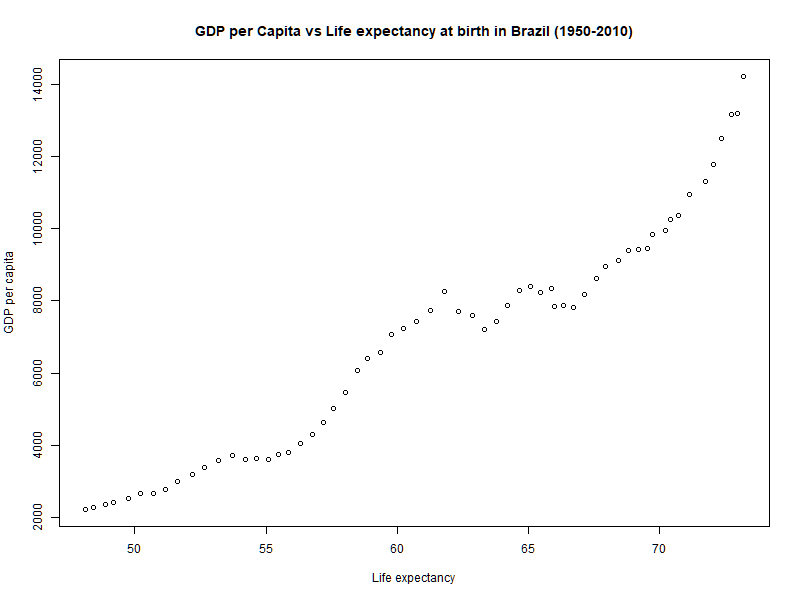
\includegraphics[width=0.95\textwidth]{tablesfolder/meu_grafico.png}

\subsection{Probability Models for two variables}

\subsubsection{Discrete Bi-variate Probability Distribution}
First, let show a table of a discrete bi-variate probability distribution.

\begin{table}[H]
\centering
\caption*{TABLE : A bivariate probability distribution}
\begin{tabular}{c|c|c|c|c}
 & \(X_1\) & \(\ldots\) & \(X_i\) & Marginal probability \\
\hline
\(Y_1\) & \(p_{11}\) & \(\ldots\) & \(p_{i1}\) & \(p_{.1}\) \\
\(\vdots\) & \(\vdots\) & \(\ddots\) & \(\vdots\) & \(\vdots\) \\
\(Y_j\) & \(p_{1j}\) & \(\ldots\) & \(p_{ij}\) & \(P_.j\) \\
\(\vdots\) & \(\vdots\) & \(\ddots\) & \(\vdots\) & \(\vdots\) \\
\(Y_p\) & \(p_{1p}\) & \(\ldots\) & \(p_{ip}\) & \(P_.p\) \\
\hline
Marginal probability & \(p_{1.}\) & \(\ldots\) & \(p_{i.}\) & 1
\end{tabular}
\end{table}

The covariance is: 

\[\sigma_{X,Y}=cov(X,Y)=E[(X-\mu_x)(Y-\mu_y)]=\displaystyle\sum_{i}\displaystyle\sum_{j}p_{ij}(X_i-\mu_x)(Y_j-\mu_y)\]

The population correlation coefficient is defined as:


\[corr(X,Y)=\rho=\frac{\sigma_{xy}}{\sigma_x\sigma_y}\]

\subsubsection{Conditional Probabilities}
Consider the \(X_i\) column in the the table above. Each cell probability may be divided by the column total, \(p_i.\), to give a conditional probability for Y given \(X_i\). Thus,
\[\frac{p_{ij}}{p_{i.}}=probability\,that\,Y = Y_i\,given\,that\, X = X_i = Prob(Y_j|X_i)\]

The mean of this distribution is the conditional expectation of Y, given \(X_i\), that is:

\[\mu_{y|x_i}=E(Y|X_i)=\sum_{j}(\frac{p_{ij}}{p_i.})Y_j\]

Similarly, the variance of this distribution is a conditional variance, or

\[\sigma^2_{y|x_i}=var(Y|X_i)=\sum_{j}(\frac{p_{ij}}{p_i})(Y_j-\mu_{y|x_i})^2\]


The conditional means and variances are both functions of X, so there is a set of "i" conditional means and variances. 

% latex table generated in R 4.3.2 by xtable 1.8-4 package
% Wed Feb  7 15:09:39 2024
\begin{table}[ht]
\centering
\caption*{Columns refer to Income (X) and rows refer to Vacation Expenditure (Y)}
\begin{tabular}{rrrr}
  \hline
 & 20000 & 30000 & 40000 \\ 
  \hline
1000 & 0.28 & 0.03 & 0.00 \\ 
  2000 & 0.08 & 0.15 & 0.03 \\ 
  3000 & 0.04 & 0.06 & 0.06 \\ 
  4000 & 0.00 & 0.06 & 0.15 \\ 
  5000 & 0.00 & 0.00 & 0.03 \\ 
  6000 & 0.00 & 0.00 & 0.03 \\ 
  Marginal Probability & 0.40 & 0.30 & 0.30 \\ 
  Mean(Y$|$X) & 1.40 & 2.50 & 3.90 \\ 
  Var(Y$|$X) & 0.44 & 0.85 & 1.09 \\ 
   \hline
\end{tabular}
\end{table}

From the table above, come the conditional probabilities:


% latex table generated in R 4.3.2 by xtable 1.8-4 package
% Wed Feb  7 17:34:32 2024
\begin{table}[ht]
\centering
\caption*{Table: Conditional Probabilities. Columns refer to Income (X) and rows refer to Vacation Expenditure (Y).}
\begin{tabular}{rrrrrrr}
  \hline
 & 1000 & 2000 & 3000 & 4000 & 5000 & 6000 \\ 
  \hline
20000 & 0.70 & 0.20 & 0.10 & 0.00 & 0.00 & 0.00 \\ 
  30000 & 0.10 & 0.50 & 0.20 & 0.20 & 0.00 & 0.00 \\ 
  40000 & 0.00 & 0.10 & 0.20 & 0.50 & 0.10 & 0.10 \\ 
   \hline
\end{tabular}
\end{table}


Using the table of conditional probabilities, it's possible to calculate the last two lines of the first table: the conditional means and variances.
\subsection{End of first part and considerations}
Certainly, there are additional statistical concepts necessary to fully understand linear regression, which is the core of Econometrics 1. If needed for any demonstration, I will incorporate these concepts into the text. The initial part of this document is derived from the book mentioned in the introduction. For now, I will likely focus on linear regression using the class notes.

In addition to these, understanding the following concepts is also necessary: the density function of probability; knowledge of well-known distributions such as Normal, Bernoulli, and Uniform; the expected value of a continuous variable; the conditional expectation of continuous variables; and matrices, including fundamental operations like sum, multiplication, and diagonalization.

\section{Linear Regression Model}
The main objective here will not be to present a formal approach to econometrics. Instead, I will aim to provide a concise overview of the theory necessary to understand the topic, and proceed with practical examples using R, Excel, and other tools.

\subsection{The k-variable model}
For this part, I am going to use class notes and \href{https://www.statlect.com/fundamentals-of-statistics/linear-regression}{statlect by Marcos Taboga}. 











\end{document}

